%% abtex2-modelo-artigo.tex, v-1.9.7 laurocesar
%% Copyright 2012-2018 by abnTeX2 group at http://www.abntex.net.br/ 
%%
%% This work may be distributed and/or modified under the
%% conditions of the LaTeX Project Public License, either version 1.3
%% of this license or (at your option) any later version.
%% The latest version of this license is in
%%   http://www.latex-project.org/lppl.txt
%% and version 1.3 or later is part of all distributions of LaTeX
%% version 2005/12/01 or later.
%%
%% This work has the LPPL maintenance status `maintained'.
%% 
%% The Current Maintainer of this work is the abnTeX2 team, led
%% by Lauro César Araujo. Further information are available on 
%% http://www.abntex.net.br/
%%
%% This work consists of the files abntex2-modelo-artigo.tex and
%% abntex2-modelo-references.bib
%%

% ------------------------------------------------------------------------
% ------------------------------------------------------------------------
% abnTeX2: Modelo de Artigo Acadêmico em conformidade com
% ABNT NBR 6022:2018: Informação e documentação - Artigo em publicação 
% periódica científica - Apresentação
% ------------------------------------------------------------------------
% ------------------------------------------------------------------------

\documentclass[
	% -- opções da classe memoir --
	article,			% indica que é um artigo acadêmico
	11pt,				% tamanho da fonte
	oneside,			% para impressão apenas no recto. Oposto a twoside
	a4paper,			% tamanho do papel. 
	% -- opções da classe abntex2 --
	%chapter=TITLE,		% títulos de capítulos convertidos em letras maiúsculas
	%section=TITLE,		% títulos de seções convertidos em letras maiúsculas
	%subsection=TITLE,	% títulos de subseções convertidos em letras maiúsculas
	%subsubsection=TITLE % títulos de subsubseções convertidos em letras maiúsculas
	% -- opções do pacote babel --
	english,			% idioma adicional para hifenização
	brazil,				% o último idioma é o principal do documento
	sumario=tradicional
	]{abntex2}


% ---
% PACOTES
% ---

% ---
% Pacotes fundamentais 
% ---
\usepackage{lmodern}			% Usa a fonte Latin Modern
\usepackage[T1]{fontenc}		% Selecao de codigos de fonte.
\usepackage[utf8]{inputenc}		% Codificacao do documento (conversão automática dos acentos)
\usepackage{indentfirst}		% Indenta o primeiro parágrafo de cada seção.
\usepackage{nomencl} 			% Lista de simbolos
\usepackage{color}				% Controle das cores
\usepackage{graphicx}			% Inclusão de gráficos
\usepackage{microtype} 			% para melhorias de justificação
% ---
		
% ---
% Pacotes adicionais, usados apenas no âmbito do Modelo Canônico do abnteX2
% ---
\usepackage{lipsum}				% para geração de dummy text
% ---
		
% ---
% Pacotes de citações
% ---
\usepackage[brazilian,hyperpageref]{backref}	 % Paginas com as citações na bibl
\usepackage[alf]{abntex2cite}	% Citações padrão ABNT
% ---

% ---
% Configurações do pacote backref
% Usado sem a opção hyperpageref de backref
\renewcommand{\backrefpagesname}{Citado na(s) página(s):~}
% Texto padrão antes do número das páginas
\renewcommand{\backref}{}
% Define os textos da citação
\renewcommand*{\backrefalt}[4]{
	\ifcase #1 %
		Nenhuma citação no texto.%
	\or
		Citado na página #2.%
	\else
		Citado #1 vezes nas páginas #2.%
	\fi}%
% ---

% --- Informações de dados para CAPA e FOLHA DE ROSTO ---
\titulo{Previsão de cotação de ações da bolsa de valores usando redes neurais recorrentes - RNN}
\tituloestrangeiro{Stock Market Forecasting Using Recurrent Neural Networks - RNN}

\autor{
	Lucas Mrowskovsy Paim\thanks{Programa de Pós Graduação em Inteligência Aritificial, Curitiba - PR, 80215-901; Especializando em Inteligência Artificial Aplicada na PUCPR; Tecnólogo em Sistemas para Internet pela Universidade Positivo; E-mail: lucasmpaim1@gmail.com} 
}

\local{Brasil}
\data{2019}
% ---

% ---
% Configurações de aparência do PDF final

% alterando o aspecto da cor azul
\definecolor{blue}{RGB}{41,5,195}

% informações do PDF
\makeatletter
\hypersetup{
     	%pagebackref=true,
		pdftitle={\@title}, 
		pdfauthor={\@author},
    	pdfsubject={Modelo de artigo científico com abnTeX2},
	    pdfcreator={LaTeX with abnTeX2},
		pdfkeywords={abnt}{latex}{abntex}{abntex2}{atigo científico}, 
		colorlinks=true,       		% false: boxed links; true: colored links
    	linkcolor=blue,          	% color of internal links
    	citecolor=blue,        		% color of links to bibliography
    	filecolor=magenta,      		% color of file links
		urlcolor=blue,
		bookmarksdepth=4
}
\makeatother
% --- 

% ---
% compila o indice
% ---
\makeindex
% ---

% ---
% Altera as margens padrões
% ---
\setlrmarginsandblock{3cm}{3cm}{*}
\setulmarginsandblock{3cm}{3cm}{*}
\checkandfixthelayout
% ---

% --- 
% Espaçamentos entre linhas e parágrafos 
% --- 

% O tamanho do parágrafo é dado por:
\setlength{\parindent}{1.3cm}

% Controle do espaçamento entre um parágrafo e outro:
\setlength{\parskip}{0.2cm}  % tente também \onelineskip

% Espaçamento simples
\SingleSpacing


% ----
% Início do documento
% ----
\begin{document}

% Seleciona o idioma do documento (conforme pacotes do babel)
%\selectlanguage{english}
\selectlanguage{brazil}

% Retira espaço extra obsoleto entre as frases.
\frenchspacing 

% ----------------------------------------------------------
% ELEMENTOS PRÉ-TEXTUAIS
% ----------------------------------------------------------

%---
%
% Se desejar escrever o artigo em duas colunas, descomente a linha abaixo
% e a linha com o texto ``FIM DE ARTIGO EM DUAS COLUNAS''.
% \twocolumn[    		% INICIO DE ARTIGO EM DUAS COLUNAS
%
%---

% página de titulo principal (obrigatório)
\maketitle


% titulo em outro idioma (opcional)



% resumo em português
\begin{resumoumacoluna}
 Este trabalho tem por objetivo criar uma rede neural de aprendizagem profunda para prever valores futuros de um papel na bolsa de valores, o papel escolhido foi PETR4 (Petrobras). A biblioteca utilizada para a criação das hipóteses foi a tensorflow, que segundo \citeonline{handsOnML}, é uma ótima biblioteca para cálculo número de código aberto,  (adicionar resultados)
 \vspace{\onelineskip}
 
 \noindent
 \textbf{Palavras-chave}: deep-learning. tensorflow. rnn. séries temporais.
\end{resumoumacoluna}


% resumo em inglês
\renewcommand{\resumoname}{Abstract}
\begin{resumoumacoluna}
 \begin{otherlanguage*}{english}
This work aims to create a deep learning neural network to predict future values of a role in the stock exchange, the role chosen was PETR4 (Petrobras). The library used for hypothesis creation was tensorflow, which according to \citeonline{handsOnML}, is a great open source number library

   \vspace{\onelineskip}
 
   \noindent
   \textbf{Keywords}:deep-learning. tensorflow. rnn. temporal series.
 \end{otherlanguage*}  
\end{resumoumacoluna}

% ]  				% FIM DE ARTIGO EM DUAS COLUNAS
% ---

% ----------------------------------------------------------
% ELEMENTOS TEXTUAIS
% ----------------------------------------------------------
\textual

% ----------------------------------------------------------
% Introdução
% ----------------------------------------------------------
\section{Introdução}

Segundo \citeonline{time-series-analysis-2009}, uma série temporal é uma coleção de observações ao longo do tempo, isto é, são dados que variam de acordo com o passar do tempo, como: comportamentos cerebrais \citeonline{NIPS2014_5624}, identificação de ritmos musicais, auxílio na composições musicais \citeonline{sbcm-2007-26}, taxa mensal de desemprego, eletrocardiograma, etc. As redes neurais recorrentes tentam identificar estes padrões fazendo conexões com neurônios anteriores. Este trabalho irá utilizar redes neurais com aprendizagem profunda, para tentar prever os valores futuros das cotações do papel PETR4 (Petrobrás), usando dados extraídos do Google Finance, com dados a partir de 2006.

% ----------------------------------------------------------
% Seção de explicações
% ----------------------------------------------------------
\section{Método}

A base utilizada para este trabalho, foram os dados históricos das ações da Petrobrás (PETR4) extraídos a partir do google finance, para o período de 05/09/2006 até 07/11/2019, estes dados podem ser visualizados na \autoref{petr4-chart}.

Utilizando a bibiloteca tensorflow (v. 2.0.0), foi montada uma rede neural recorrente (RNN), utilizando duas camadas de neurônios de memória LSTM (Long Short Term Memory), o modelo gerado pode ser consultado na imagem: \autoref{model-image}

Em um primeiro momento, a base foi dividida em teste e validação em que os últimos 6 valores da base foram separados em: 5 para dados e 1 previsão e o resto da base é utilizada para treinamento, em que também é dividida na proporção 5:1 e treinada durante 100 épocas, estas configurações foram escolhidas empiricamente , para a escolha desses hiperparâmetros, uma abordagem melhor seria com o uso de algoritmos de busca como os algoritmos genéticos.

O gráfico de loss durante o treinamento, comparando a base de validação e a de treinamento pode ser visualizada na \autoref{loss-graph}, nele podemos notar que não houve overitting na rede, as camadas "Dropout" que aparecem na \autoref{model-image} que segundo \citeonline{dropout} definindo aleatoriamente as arestas de saída das neurônios ocultos como 0.

As células LSTM, proposta em 1997 por Sepp Hochreiter e Jurgen Schmidhuber e aperfeiçoada desde então, que segundo \citeonline{handsOnML}, sua ideia-chave é que a rede possa aprender o que armazenar a longo prazo durante o treinamento.

Para a avialiação do erro foi utilizado a métrica MAE (Mean Absoluty Error), que é a média aritmética da diferença entre o valor previsto e o valor real, ela pode ser representada pela fórmula:

\begin{equation}
mae = \frac{1}{n}\sum_{i=0}^M |{y_1 - y^*_i}|
\end{equation}

O modelo atingiu uma MSE de 

% ----------------------------------------------------------
% ELEMENTOS PÓS-TEXTUAIS
% ----------------------------------------------------------
\postextual

% ----------------------------------------------------------
% Referências bibliográficas
% ----------------------------------------------------------
\bibliography{references}

% ----------------------------------------------------------
% Glossário
% ----------------------------------------------------------
%
% Há diversas soluções prontas para glossário em LaTeX. 
% Consulte o manual do abnTeX2 para obter sugestões.
%
%\glossary

% ----------------------------------------------------------
% Apêndices
% ----------------------------------------------------------


% ----------------------------------------------------------
% Anexos
% ----------------------------------------------------------
\cftinserthook{toc}{AAA}
% ---
% Inicia os anexos
% ---
%\anexos
\begin{anexosenv}

\begin{figure}[htb]
	\caption{\label{petr4-chart}Gráfico histórico PETR4 R\$ x Dias úteis após 05/09/2006}
	\begin{center}
		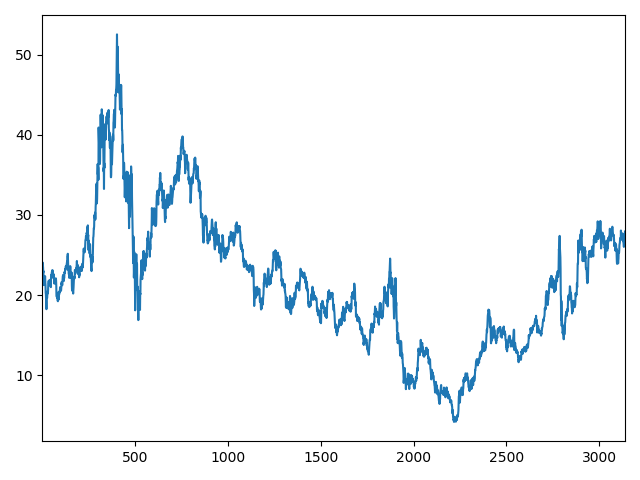
\includegraphics[scale=0.5]{images/petr4_chart.png}
	\end{center}
	\legend{Fonte: O Autor}
\end{figure}

\begin{figure}[htb]
	\caption{\label{model-image}Modelo}
	\begin{center}
		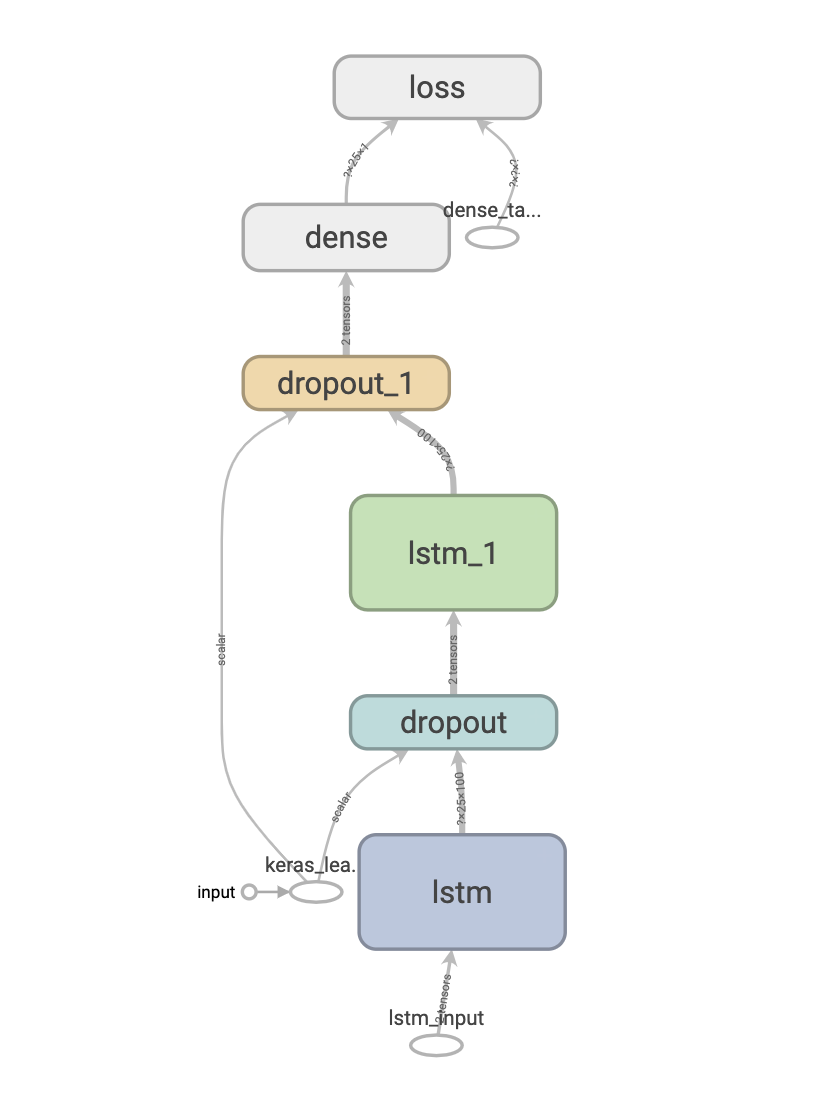
\includegraphics[scale=0.5]{images/model.png}
	\end{center}
	\legend{Fonte: O Autor}
\end{figure}

\begin{figure}[htb]
	\caption{\label{loss-graph}Loss}
	\begin{center}
		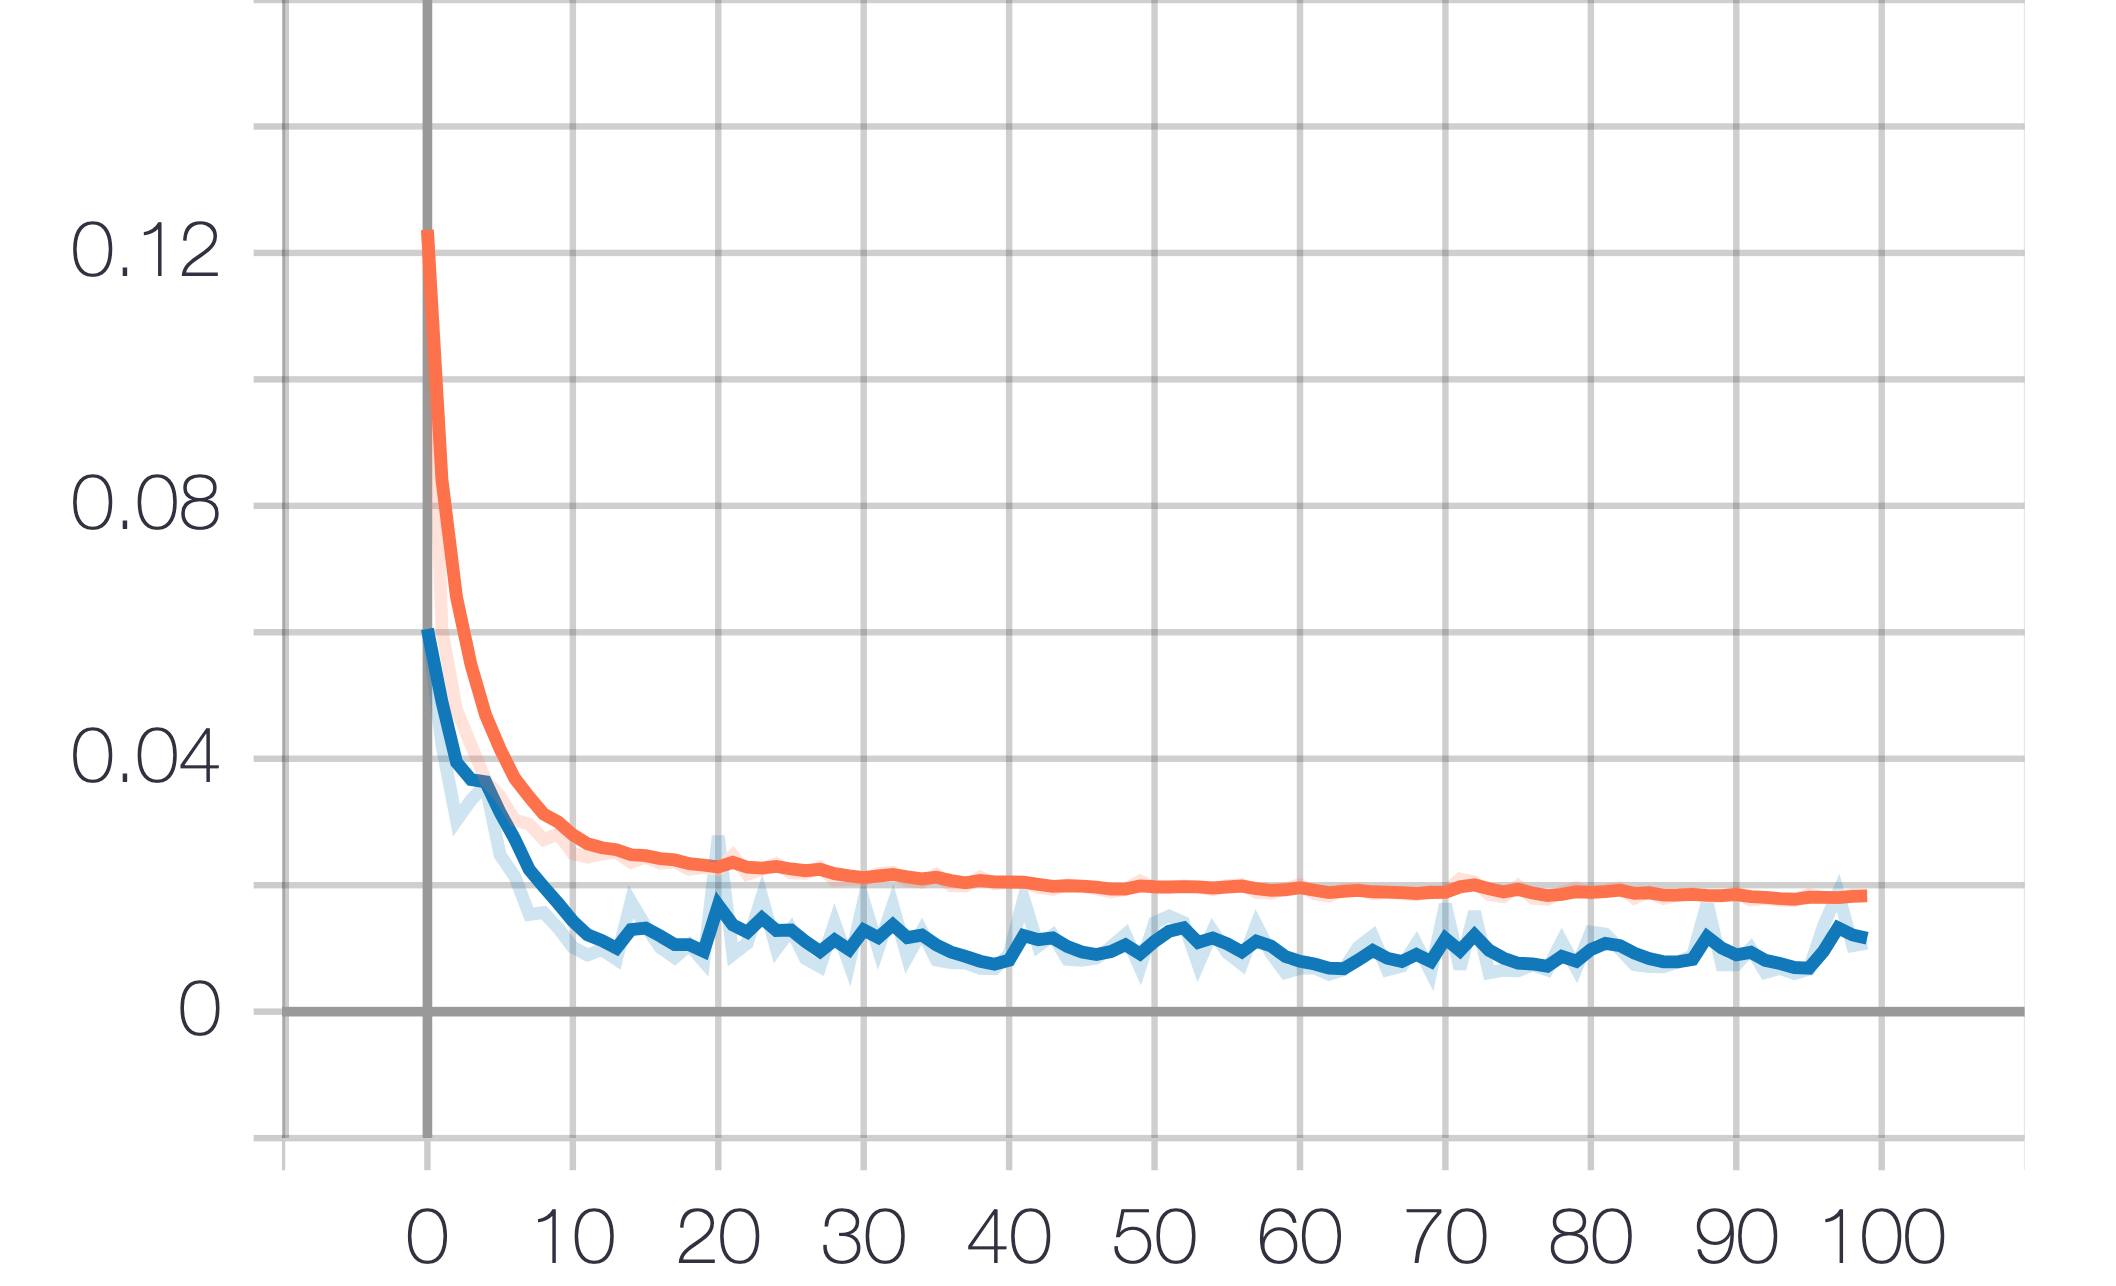
\includegraphics[scale=0.5]{images/loss.png}
	\end{center}
	\legend{Fonte: O Autor}
\end{figure}


\end{anexosenv}


\end{document}
